\section{Related Work}

The use of scientific visualization in immersive environments is simply natural while tactically important for scientific discovery, product design and data analysis.
There are several high-quality scientific visualization VR applications created from scratch using OpenGL directly~\cite{Billen:2008, LaViola:2007, Schulze:2001, Rantzau:1998} such as the stunning graphics processing unit (GPU) accelerated hybrid volume and glyph approach for molecular dynamics and other visualizations in the CAVE2\texttrademark~\cite{Reda:2013, Reda:2013a}.
These are certainly exemplary and valuable applications.
When building immersive applications with scientific visualization requirements, much like when building desktop applications, it is often more efficient to leverage the open-source visualization toolkit (VTK)~\cite{Schroeder:2004}.

Throughout the past two decades, several research teams and developers have integrated VTK with immersive environments to varying degrees of success.
Four fundamental approaches are available to enable VTK in an immersive system:

\begin{compactitem}
\item geometry transport;
\item OpenGL context sharing;
\item VR toolkit embedding; and
\item OpenGL intercept.
\end{compactitem}

Our recent enhancements to the VTK platform contain solutions for the desired integration that present a number of contributions. Therefore, we review related work for these areas.

\textbf{\textit{Geometry transport}}
An early approach to VTK-VR integration was to use the \texttt{vtkActorToPF} library~\cite{Leigh98limbo/vtk}.
In this approach, the generation of visualization geometry is decoupled from
the rendering of the geometry. (See Figure~\ref{fig:vtkActorToPF}.) 
The geometry is generated by VTK in the form of actors that consist of polygons and properties.
\texttt{vtkActorToPF} transforms these actors into pf-Geodes (nodes) that are included in a Performer (or OpenSceneGraph) scene graph. The geometry is created by VTK, and the scene graph is rendered without VTK. Only geometry is transformed. Cameras, lights, rendering and interaction are not incorporated. Several applications utilized the equivalent \texttt{vtkActorToOSG} for an OpenSceneGraph-based scene graph~\cite{VE-Suite:2016} or directly into OpenGL~\cite{Ohno:2006}. Others have used VTK in a preprocessing step to produce geometries or textures eliminating the need for a direct connection to VTK~\cite{Bivins:2005}.

\begin{figure}[h!]
  \centering
  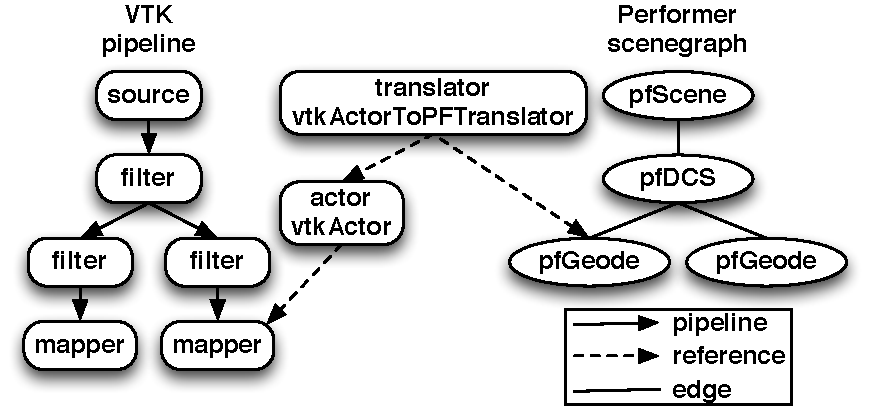
\includegraphics[width=\linewidth]{images/vtkActorToPF.pdf}
  \caption{VTK, vtkActorToPF and Performer interaction diagram. (Recreated from Paul Rajlich~\cite{Leigh98limbo/vtk}.)}
  \label{fig:vtkActorToPF}
\end{figure}

VTK can be used to create, transport and save geometry without rendering. As effective as this approach can be, the loose coupling of VTK and the VR toolkit creates more obstacles than benefits from an application developer's perspective. The approach is, therefore, not built upon by this work.

\textbf{\textit{OpenGL context sharing}} Rather than share just the VTK geometry, the application developer would like to use all of the VTK API from within his or her immersive application.
In VTK, the renderer and render window classes are responsible for rendering scenes.
VTK creates its own window and associates an OpenGL context with that window for the renderer to use.
The following lists what an OpenGL context represents: all of the state; the default framebuffer; and everything affiliated with OpenGL with respect to the renderer, the window and the application.
The application developer seeks to simply share the OpenGL context from the VR toolkit with a third-party rendering software (e.g. Delta3D~\cite{McDowell:2006}, OpenSceneGraph~\cite{Wang:2010} and VTK). 

In previous work by Sherman et al.~\cite{Sherman:2010} and others, Delta3D
and OpenSceneGraph were quickly modified to instead use the windows and the associated
OpenGL contexts of a VR integration library such as Vrui~\cite{Kreylos:2006}.  
% in final paper can mention FreeVR.
OmegaLib~\cite{Febretti:2014} software for hybrid reality display environments also implements its own OpenGL context-sharing module for VTK, \texttt{omegaVtk}. The AlloSystem~\cite{Amatriain:2009} for the AlloSphere Research Facility originally had an OpenGL context-sharing VTK plugin, but it has recently (October 2016) changed to our \texttt{vtkRenderingExternal} VTK module, which is presented in this paper.
These solutions are generally limited in their integration.
Specifically, a rendering library that is unaware of the actual
viewing matrix does not calculate lighting correctly, and
picking input operations do not conform to the shifted rendering. As the VTK API adapts and adds enhancements in time, these implementations are generally locked in to older versions of VTK.

Our \texttt{vtkRenderingExternal} VTK module formalizes this integration, providing lights, interaction and picking connectivity that are lacking in other implementations. The module also offers the application developer complete access to the VTK pipeline.

\textbf{\textit{VR toolkit embedding}} A similarly time-proven approach is based on the modification of the VTK renderer and render window~\cite{van2000vista, Hannema:2001, Shamonin02vtkcave, Belleman:2003}. 
To render in an immersive environment, derived classes of
\texttt{vtkRenderer} and \texttt{vtkRenderWindow} are created, which depend on fundamental calls to the VR toolkit.
Thus, VTK based applications can simply exchange these two items to run on the desktop or the immersive environment.
\texttt{vtkCave}~\cite{Tufo:1999} for the CAVELib~\cite{CAVELib:2016}, followed by
\textt{vjVTK}~\cite{Blom:2006} and VR JuggLua~\cite{Pavlik:2012} for
VRJuggler~\cite{Bierbaum:2001}, created third-party software, essentially
deriving the \texttt{vtkRenderWindow} and \texttt{vtkRenderer} classes. Outside of VTK, lighting and interaction were not shared, which resulted in troublesome behavior.

In this work, we have created two new VTK modules based on either the Oculus~\cite{Oculus:2016} or the OpenVR~\cite{OpenVR:2016} software development kits (SDKs).
OpenVR is an API developed by Valve to support its SteamVR ecosystem that is compatible with the HTC Vive and other VR hardware~\cite{Road2VR:2015}. Oculus provides software development kits more closely tied to its equipment for mobile, desktop and web VR. The Oculus and OpenVR VTK modules directly support several immersive environments
without the issues faced by previous work. These modules provide a complete template
for embedding other VR toolkits within VTK in future work.

\textit{\textbf{OpenGL intercept}}
A fourth possible means for melding VTK into a virtual environment system
is the \textit{OpenGL intercept} method
~\cite{Humphreys:2001,Humphreys:2002,Zielinski:2014,TechViz:2016,Conduit:2016}, in which middleware is inserted between the application and the graphics card at runtime.
With this technique, closed-source applications can be rendered so that
the head-tracked perspective rendering overrides the internal view matrix
to provide the VR experience.
Thus, this technique enables basic desktop tools to be used with an
immersive interface|albeit a limited interface, given the open-loop nature of
grabbing the rendering but not connecting back to the parameter interface.
Yet, the perspective rendering alone can be extremely valuable and can allow
scientists, engineers or medical researchers to interact with their desktop
tools in a whole new way. Many of these methods, however lack full functionality in immersive environments, which limits their usefulness to end users.
Pure OpenGL, without any modifications or additions, is sure to work with interception.
The difficulties of using intercept methods are that they require more coding
and tagging, and they are not guaranteed to work at all. These difficulties are becoming
more apparent with OpenGL 3.0+, especially when using a core OpenGL profile.

In contrast to the OpenGL intercept method, the work in this paper is for the application developer, and there is no intention to eliminate the need to write code. This work aims to make  it easier to develop scientific visualization immersive applications by leveraging VTK.

\textit{\textbf{Enhanced performance}} Near real-time update of scientific visualization metaphors is crucial in immersive environments.
The field has seen several proposed solutions from decoupling rendering and processing to parallel visualization~\cite{Bryson:1996, van2000vista}.
This effort stands apart from all these previous efforts. Valiant
as they were, the efforts were ultimately lost to time, as VTK has continued to
evolve, making it difficult for tacked-together components to remain in
sync with the API.
Rather, by providing rendering access from within the VTK API itself, new
tools can rely on a stability that has not been available for techniques
that perform functions outside the bounds of the API design. Often, such techniques access
internal features that do not have the assurance of stability.
As a commercially supported open-source tool, the rendering performance of VTK is
continually being advanced.
VTK has been around since 1993. The toolkit has over 100,000 repository commits from more than 250 contributors.
Having the latest algorithm implementation requires using the existing implementation in VTK or contributing the algorithm to VTK.

We present recent enhancements to VTK that significantly impact immersive
environment application development. The OpenGL 3.2+ pipeline, described in Hanwell et al~\cite{Hanwell:2015}, provides the most dramatic improvement in performance. We have supplemented this work with Bavoil and Myers dual depth peeling~\cite{Bavoil:2008}, as well as with symmetric multiprocessing (SMP) tools and algorithms, to address the performance issues for transparent geometry and computationally intense algorithms (e.g., isosurfaces).

Finally, our work will eventually allow application developers to leverage portable, threaded data parallel algorithms that are capable of running on next-generation hardware from VTK-m~\cite{Moreland:2016}. VTK-m has shown impressive results in its first two years of development. We plan to make the filters in the VTK-m repository available in the next major release of VTK. Thus, if VTK-m is contained in VTK, then applications developed with the integrations described in this paper can use VTK-m.
